\documentclass[12pt,twoside,space]{ctexart}
\usepackage{NEMT}
\usepackage{float}
\begin{document}\zihao{5}
\juemi
\biaoti{全国高考一卷}
\fubiaoti{理科数学}
{\heiti 注意事项}
\begin{enumerate}[itemsep=-0.3em,topsep=0pt]
\item 答卷前,考生务必将自己的姓名和准考证号填写在答题卡上。
\item 回答选择题时,选出每小题答案后,用铅笔把答题卡对应题目的答案标号涂黑。如需改动,用橡皮擦干净后,再选涂其它答案标号。回答非选择题时,将答案写在答题卡上。写在本试卷上无效。
\item 考试结束后,将本试卷和答题卡一并交回。
	请认真核对监考员在答题卡上所粘贴的条形码上的姓名、准考证号与您本人是否相符。
\end{enumerate}
\section{选择题:本题共3个小题,共6分}
\begin{enumerate}[itemsep=0.2em,topsep=0pt]
\item
一道考题有4个答案,要求学生将其中的一个正确答案选择出来。某考生知道正确答案的概率为$\frac{1}{3}$,若不知正确答案,学生会乱猜。在乱猜时,4个答案被选择的概率均为$\frac{1}{4}$,如果他答对了,则他确实知道正确答案的概率是
\begin{tasks}(4)\task $\frac{1}{3}$ \task $\frac{2}{3}$ \task $\frac{3}{4}$ \task $\frac{1}{4}$ 
\end{tasks}
\item
$-5\cos(x+\varphi)=3\sin(x)+4\cos(x)$对$x\in R$恒成立,则$\sin(\varphi-\dfrac{\pi}{6})=$( ).
\begin{tasks}(4)\task $$\dfrac{4+3\sqrt{3}}{10}$$ \task $$\dfrac{3\sqrt{3}-4}{10}$$ \task $$\dfrac{4-3\sqrt{3}}{10}$$ \task $$-\dfrac{4+3\sqrt{3}}{10}$$ 
\end{tasks}
\item
已知$\alpha,\beta$是锐角,且$\cos(\alpha+\beta)=\dfrac{3}{5},\sin{\alpha}=\dfrac{5}{13}$,则$\cos{\beta}$的值为( ).
\begin{tasks}(4)\task $$\dfrac{56}{13}$$ \task $$\dfrac{33}{65}$$ \task $$\dfrac{16}{65}$$ \task $$\dfrac{63}{65}$$ 
\end{tasks}
\end{enumerate}
\section{解答题:本题共2个小题,共22分}
\begin{enumerate}[itemsep=0.2em,topsep=0pt]
\item
如图,抛物线$ y=\frac{1}{5}x^2-\frac{16}{5} $与x轴交与A,B两点,顶点为C,点P在抛物线上,且位于x轴下方。已知P(1,-3),B(4,0),若点D是抛物线上的一点,满足$ \angle DPO=\angle POB $,求点D的坐标。
\begin{figure}[H]
                      \centering
                      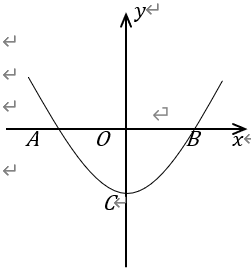
\includegraphics[width=10em]{288793-1632795205-2.jpg}
\end{figure}
\item
在$\triangle ABC$中,角$A,B,C$对应的边分别为$a,b,c$且$b=1,c=\sqrt{3},\angle C=\frac{2}{3}\pi.$(1)求$cosB$的值.(2)求$a$的值
\end{enumerate}

\clearpage
\end{document}
\documentclass{article}
\usepackage{pdfpages}
\usepackage[paperwidth=39.5cm,paperheight=27.2cm]{geometry}
\begin{document}
\includepdf[pages=1-6,nup=2x1]{dibajiefeishujuesaijuanzi.pdf}
\end{document}
doublepages